%%
%% (
%%  )\ )                             (
%%  (()/(   (            (             )\  )   (
%%   /(_))  ))\   (       ))\  (   (   (()/(   ))\
%%   (_))  /((_)  )\  )  /((_) )\  )\   ((_))/((_)
%%   | _ \(_))(  _(_/( (_) )  ((_)((_)  _| |(_))
%%   |   /| || || ' \))/ -_)/ _|/ _ \/ _` |/ -_)
%%   |_|_\ \_,_||_||_| \___|\__|\___/\__,_|\___|
%%

\documentclass{article}
\usepackage[utf8x]{inputenc}
\usepackage{amsmath}
%\usepackage{slashbox}
\usepackage{amsfonts}
\usepackage{amssymb}
\usepackage{graphicx} % Paquete para incluir imágenes en el documento LaTeX
\usepackage{hyperref}
\hypersetup{
  colorlinks=true,
  linkcolor=blue,
  filecolor=magenta,
  urlcolor=cyan,
}
\urlstyle{same}
\usepackage{varwidth}

\newcommand\tab[1][1cm]{\hspace*{#1}}

\usepackage{multirow}

\usepackage[a4paper,rmargin=1.5cm,lmargin=1.5cm,top=1.5cm,bottom=1.5cm]{geometry}

\usepackage{pdfpages}

\usepackage{xcolor}
\usepackage{minted}
\setminted[css]{frame=lines, framesep=2mm, baselinestretch=1.2, rulecolor=\color{black!80},
                bgcolor=DarkGray,fontsize=\normalsize}
\usemintedstyle[css]{monokai}
\setminted[python]{frame=lines, framesep=2mm, baselinestretch=1.2, rulecolor=\color{black!80}, bgcolor=DarkGray}
\usemintedstyle[python]{monokai}
\setminted[java]{frame=lines, framesep=2mm, baselinestretch=1.2, rulecolor=\color{black!80}, bgcolor=DarkGray}
\usemintedstyle[java]{monokai}
\setminted[javascript]{frame=lines, framesep=2mm, baselinestretch=1.2, rulecolor=\color{black!80}, bgcolor=DarkGray}
\usemintedstyle[javascript]{monokai}
\setminted[php]{frame=lines, framesep=2mm, baselinestretch=1.2, rulecolor=\color{black!30}, bgcolor=LightGray}
\setminted[html]{frame=lines, framesep=2mm, baselinestretch=1.2, rulecolor=\color{black!30}, bgcolor=LightGray}
\setminted[bash]{baselinestretch=1.2,rulecolor=\color{black!30},bgcolor=LightGray}
\definecolor{LightGray}{gray}{0.90}
\definecolor{DarkGray}{gray}{0.1}
\definecolor{MidGray}{gray}{0.8}
\definecolor{codegreen}{rgb}{0,0.6,0}
\definecolor{codegray}{rgb}{0.5,0.5,0.5}
\definecolor{codepurple}{rgb}{0.58,0,0.82}
\definecolor{backcolour}{rgb}{0.95,0.95,0.92}
\setminted[json]{frame=lines, framesep=2mm, baselinestretch=1.2, rulecolor=\color{black!80}, bgcolor=DarkGray}
\usemintedstyle[json]{monokai}
\setminted[apacheconf]{frame=lines, framesep=2mm, baselinestretch=1.2, rulecolor=\color{black!30}, bgcolor=LightGray}
\setminted[html+twig]{frame=lines, framesep=2mm, baselinestretch=1.2, rulecolor=\color{black!30}, bgcolor=LightGray}
\setminted[html+php]{frame=lines, framesep=2mm, baselinestretch=1.2, rulecolor=\color{black!30}, bgcolor=LightGray}

\setlength{\parindent}{0px}  % Setea la indentacion de la primera linea de cada parrafo a cero pixeles.


\title{Configurar Eclipse con C++}
\author{@RuneCode}

\begin{document}
%% Portada
% \includepdf{./portada/portada.pdf}

%% Introduccion
\section{Introducción}%
Hola compañeros, quería incluir esto para no tener que escribirles todo un
comentario grande en el Whatsapp xD.\\

Primero me gustaría mencionarles que Eclipse es un IDE muy bueno del que se
puede aprovechar muchas características. Yo entiendo que se complica
configurarlo y más para usarlo con C, que yo al igual que ustedes siempre lo he
trabajado con un editor simple nomás.\\

No se si han escuchado sobre \textbf{Spring Tools Suite 4}, bueno este es un IDE
usado para programar Java Spring, que es un framework para programar web con
Java (disculpas para los que ya sabían esto y les es repetitivo). Bueno Spring
Tool Suit es un IDE que se carga sobre Eclipse, así que puede valer la pena
aprender algo de este IDE chicos.\\

Y por eso es que decidí hacer este especie de tutorial con capturas para poder
documentar lo que aprendí de este IDE.

\newpage


%% Clase previa #1
\section*{Instalar soporte para C y C++ en IDE JAVA Eclipse}%
Si ya cuentas con Eclipse IDE para JAVA, puedes instalarle paquetes para que
pueda tener soporte con C y C++. Para esto se realiza lo siguiente:

\begin{figure}[h!]
  \centering
  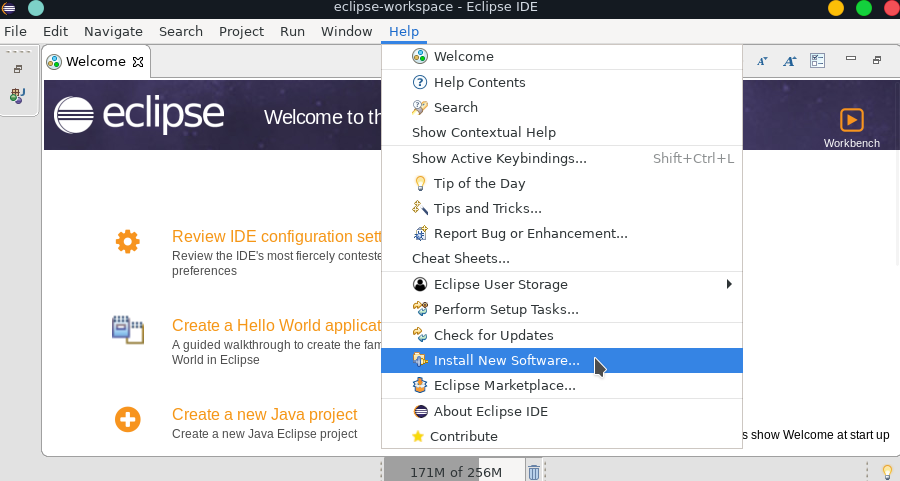
\includegraphics[scale=0.75]{./Pictures/001_eclipse_help.png}
\end{figure}

\begin{figure}[h!]
  \centering
  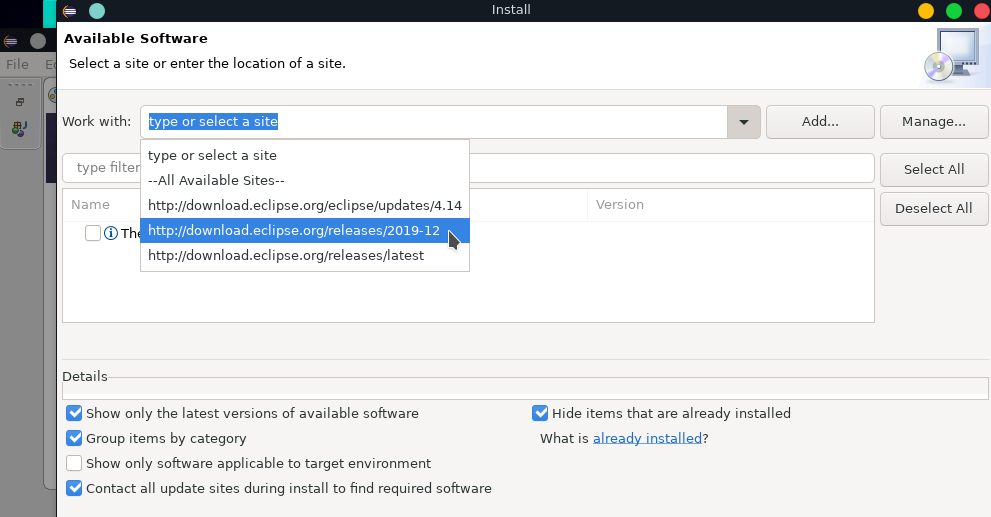
\includegraphics[scale=0.7]{./Pictures/002_eclipse_cpp_repo.png}
\end{figure}

\newpage

\begin{figure}[h!]
  \centering
  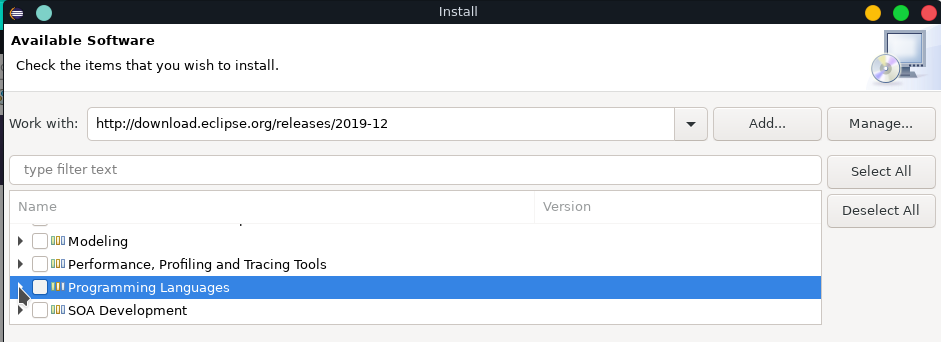
\includegraphics[scale=0.75]{./Pictures/003_programming_repo.png}
\end{figure}

\begin{figure}[h!]
  \centering
  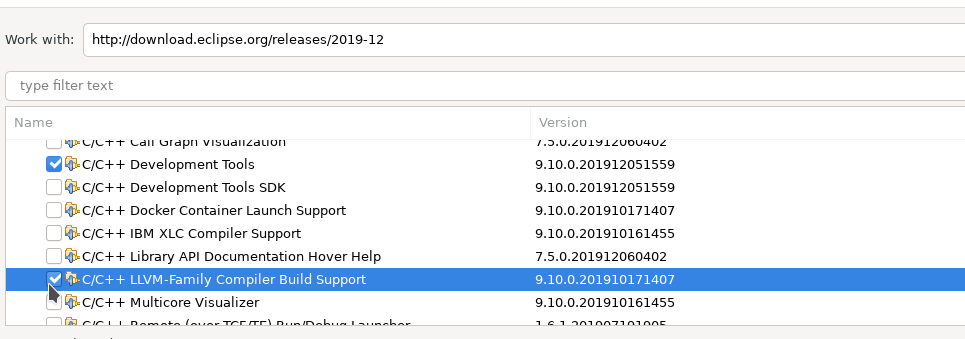
\includegraphics[scale=0.75]{./Pictures/004_paquetes.png}
\end{figure}

\begin{figure}[h!]
  \centering
  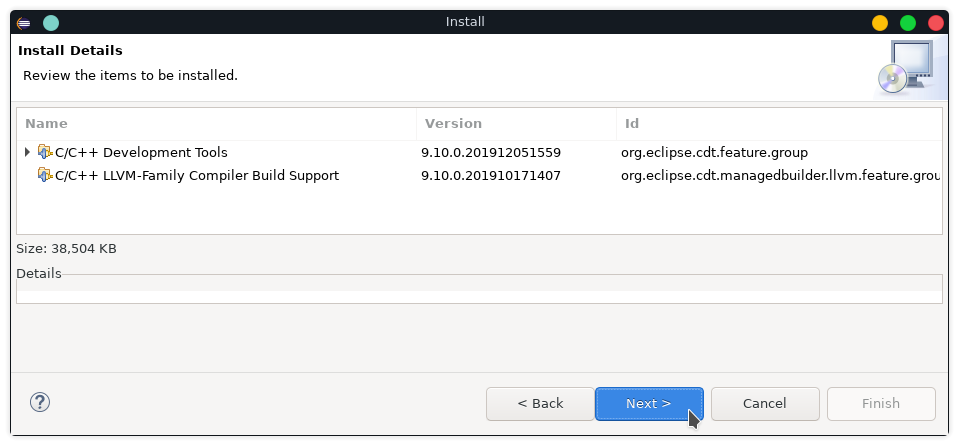
\includegraphics[scale=0.75]{./Pictures/005_next.png}
\end{figure}

\newpage

\begin{figure}[h!]
  \centering
  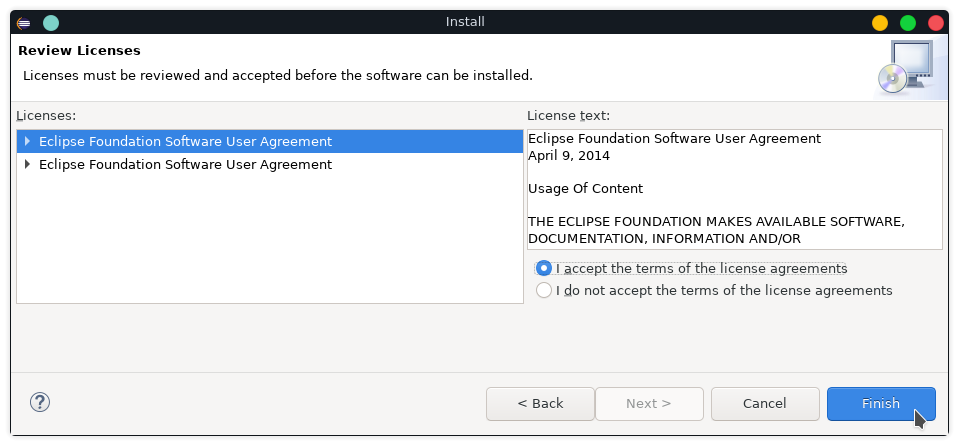
\includegraphics[scale=0.75]{./Pictures/006_aceptar_terminos.png}
\end{figure}

\begin{figure}[h!]
  \centering
  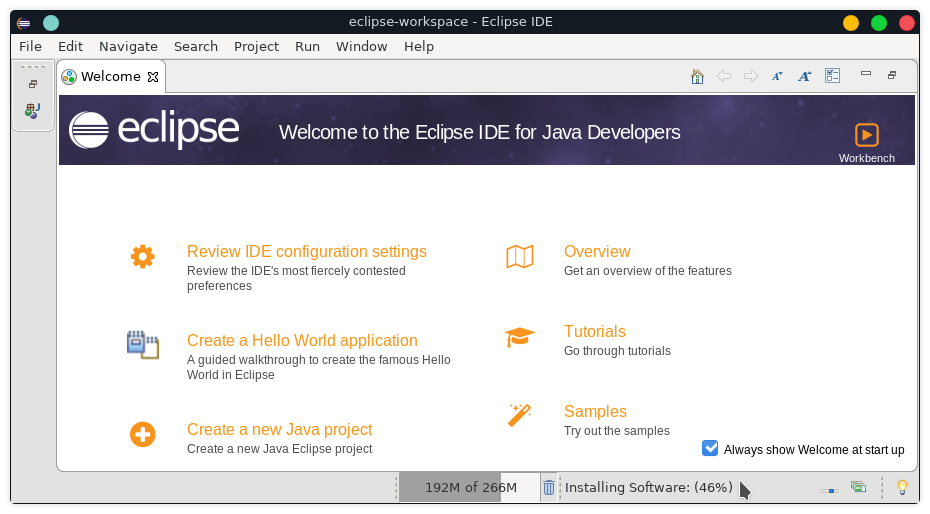
\includegraphics[scale=0.75]{./Pictures/007_instalando.png}
\end{figure}

\begin{figure}[h!]
  \centering
  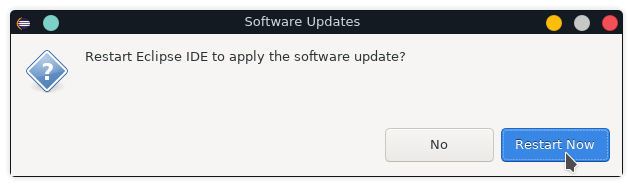
\includegraphics[scale=0.75]{./Pictures/008_restart.png}
\end{figure}

\newpage

\begin{figure}[h!]
  \centering
  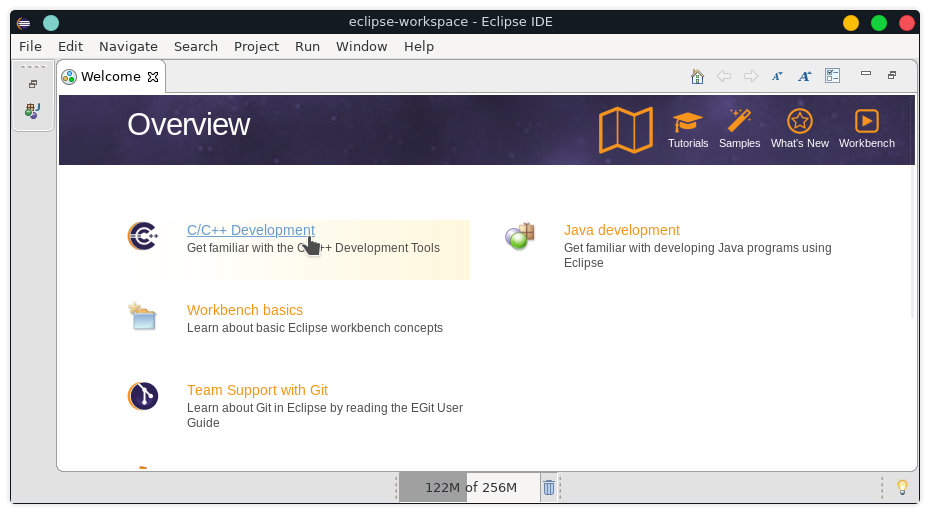
\includegraphics[scale=0.75]{./Pictures/009_reiniciado.png}
\end{figure}

\newpage


\section*{Usar un repositorio remoto git con Eclipse}%
En Eclipse puedes crear un repositorio local o clonar un repositorio remoto,
para lo segundo primero debes crear dicho repositorio en Github o cualquier
otra plataforma en la web que almacene repositorios con git.\\

Para poder gestionar los repositorios con Eclipse, contamos con un panel que no
está visible por defecto, debemos mostrarlo. Para esto hacemos lo siguiente:

\begin{figure}[h!]
  \centering
  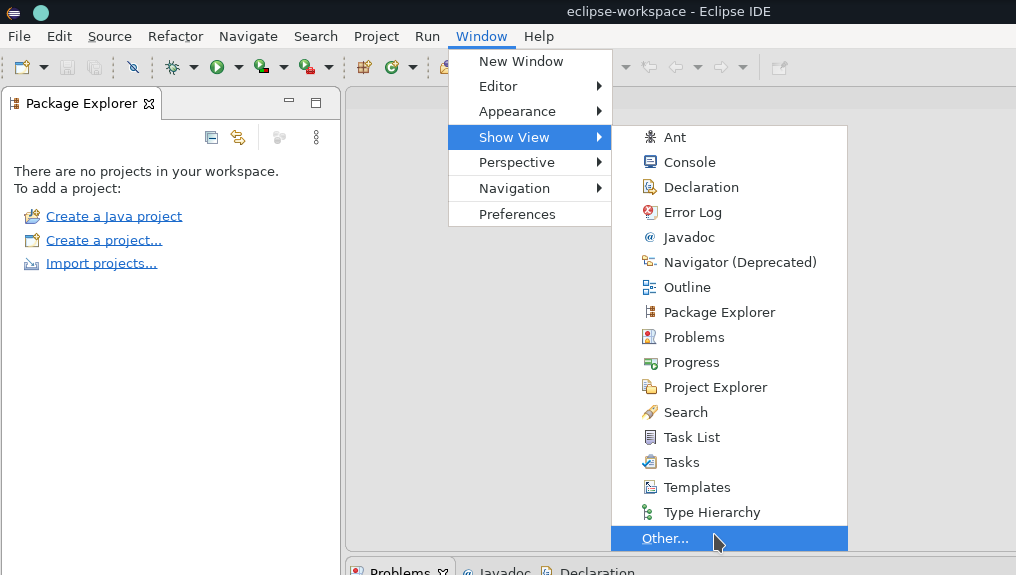
\includegraphics[scale=0.7]{./Pictures/010_other_git.png}
\end{figure}

\begin{figure}[h!]
  \centering
  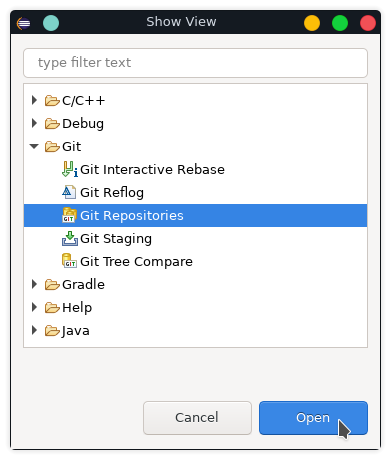
\includegraphics[scale=0.75]{./Pictures/011_show_view_git_repository.png}
\end{figure}

\newpage

\subsection*{Clonando un repositorio remoto}%
En el panel que acabmos de activar podemos, entre otras opciones, clonar un
repositorio remoto:

\begin{figure}[h!]
  \centering
  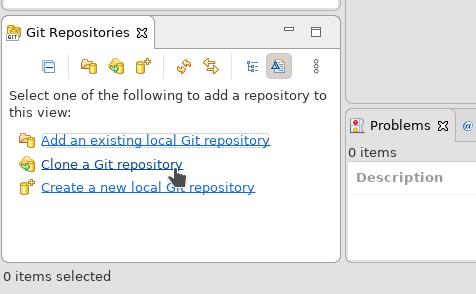
\includegraphics[scale=0.75]{./Pictures/012_clone_repository.png}
\end{figure}

Copiamos el url de clonar with HTTPS de Github (en este caso).

\begin{figure}[h!]
  \centering
  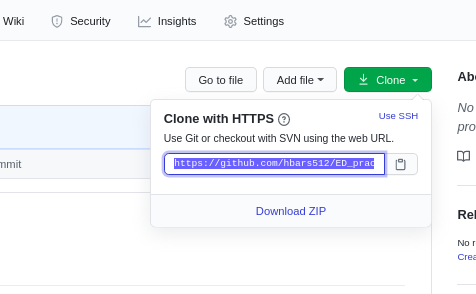
\includegraphics[scale=0.75]{./Pictures/013_link_clone.png}
\end{figure}

\newpage

Es necesario autenticarse con las credenciales de Github.

\begin{figure}[h!]
  \centering
  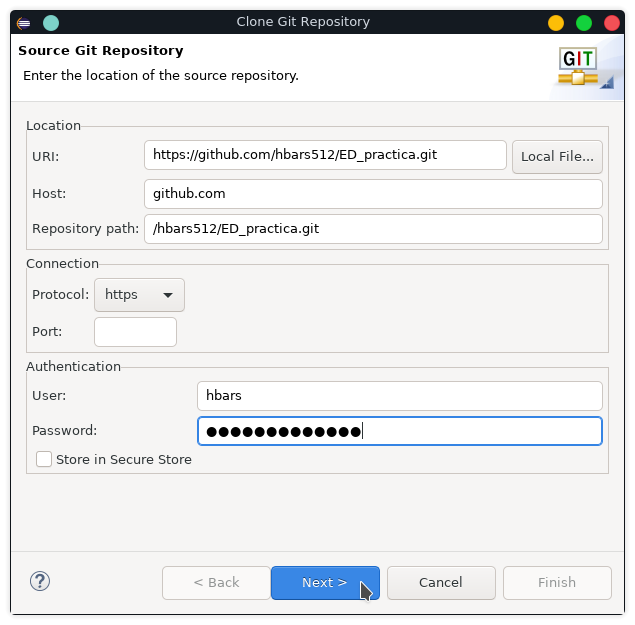
\includegraphics[scale=0.75]{./Pictures/014_source_git_repository.png}
\end{figure}

\begin{figure}[h!]
  \centering
  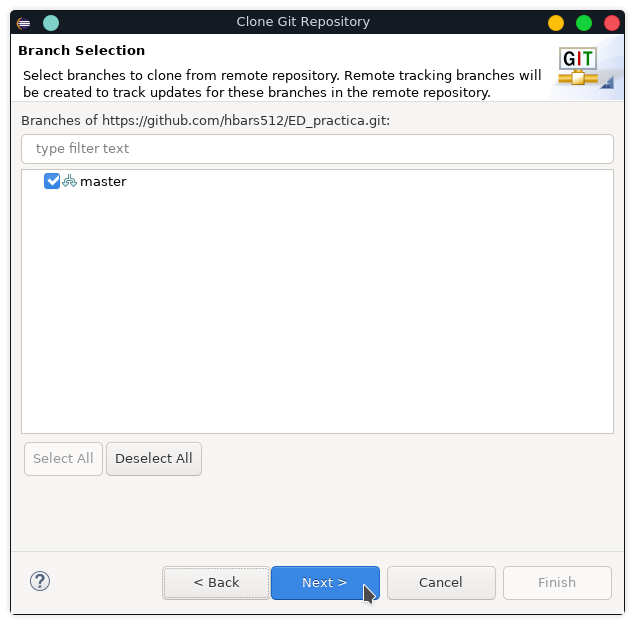
\includegraphics[scale=0.75]{./Pictures/015_source_ramas.png}
\end{figure}

\newpage

\begin{figure}[h!]
  \centering
  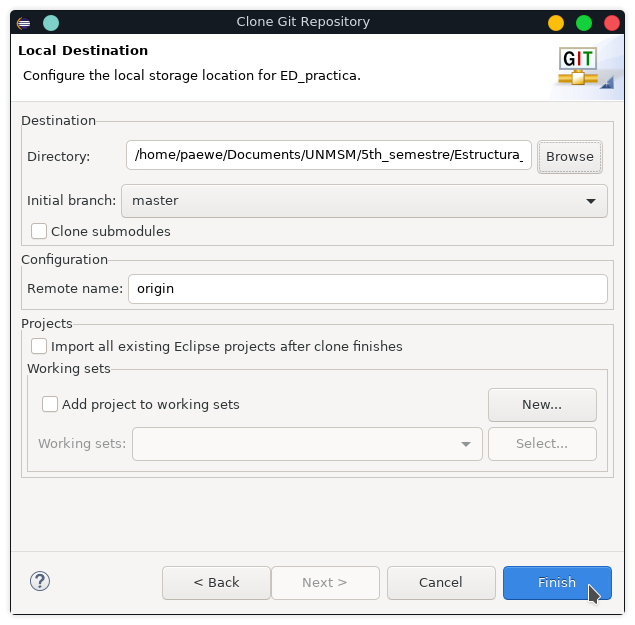
\includegraphics[scale=0.75]{./Pictures/016_local_destination.png}
\end{figure}

Hasta este punto ya tenemos el repositorio remoto en nuestra computadora (esto
es el repositorio local). Para poder trabajar el proyecto tenemos que
importarlo.

\begin{figure}[h!]
  \centering
  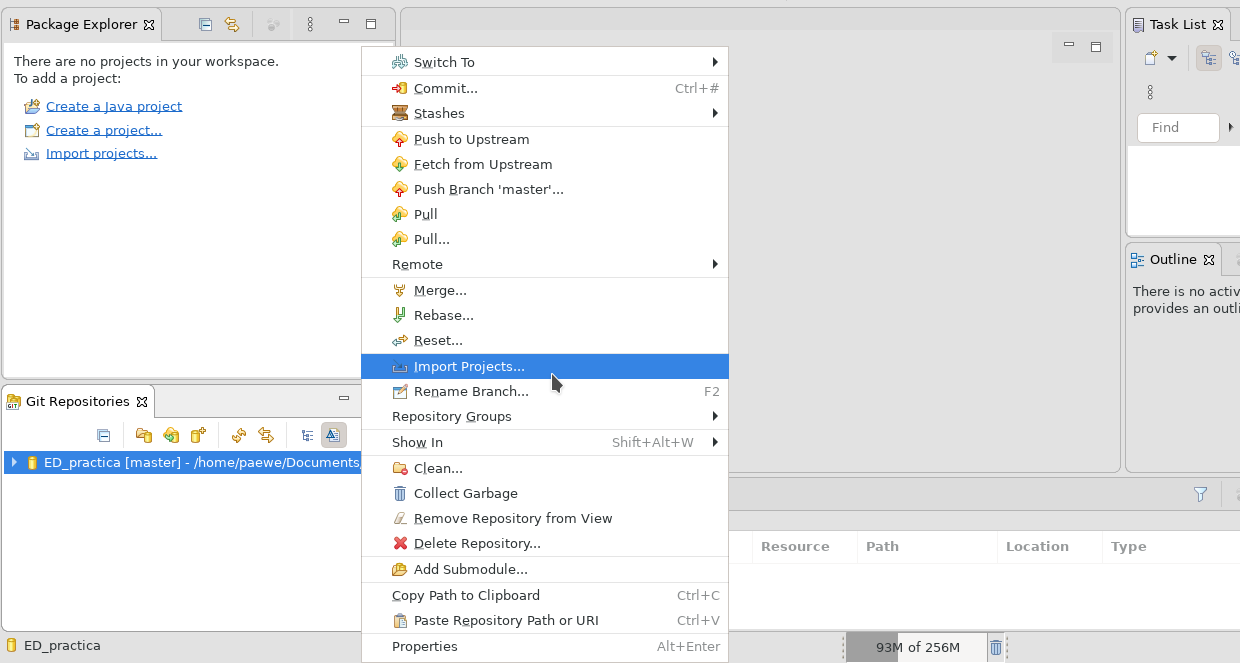
\includegraphics[scale=0.55]{./Pictures/017_importar_repo.png}
\end{figure}

\newpage

\begin{figure}[h!]
  \centering
  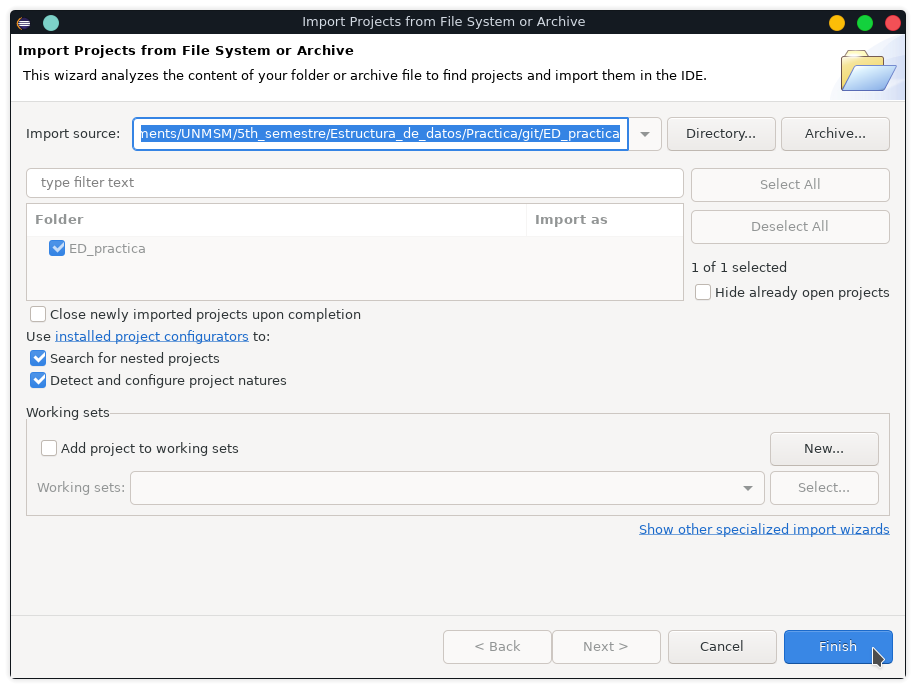
\includegraphics[scale=0.75]{./Pictures/018_save_import.png}
\end{figure}

Finalizado este proceso, ya tenemos nuestro proyecto en el Package Explorer de
Eclipse.

\begin{figure}[h!]
  \centering
  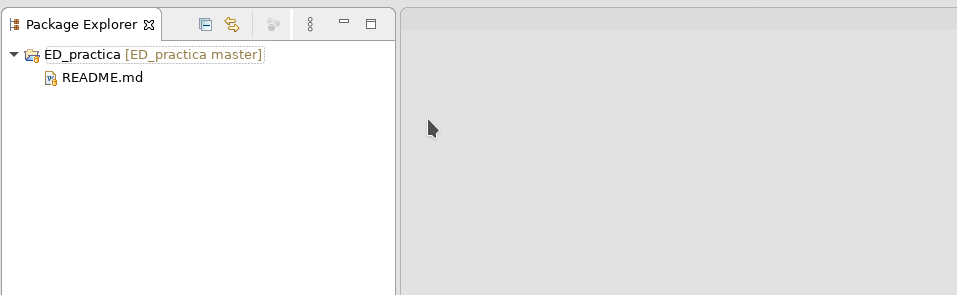
\includegraphics[scale=0.75]{./Pictures/019_project_imported.png}
\end{figure}

\newpage


\subsection*{Creando un proyecto anidado}%
En el caso específico de Estructura de Datos, revisando cómo el profesor
Herminio ha trabajado su respositorio, en este ejemplo vamos a crear proyectos
anidados por cada ejercicio.

\begin{figure}[h!]
  \centering
  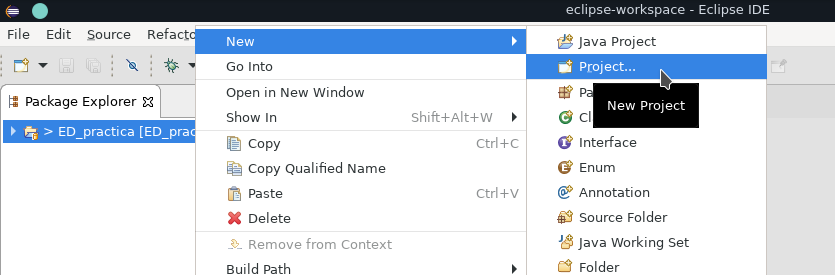
\includegraphics[scale=0.75]{./Pictures/020_new_project.png}
\end{figure}

\begin{figure}[h!]
  \centering
  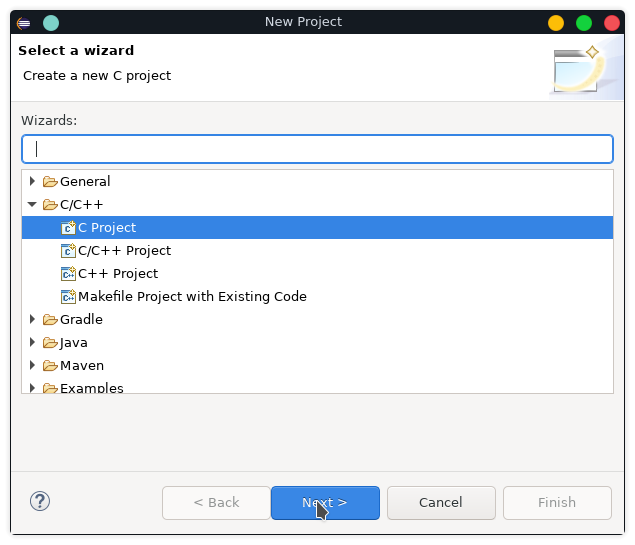
\includegraphics[scale=0.75]{./Pictures/021_c_project.png}
\end{figure}

\newpage

\begin{figure}[h!]
  \centering
  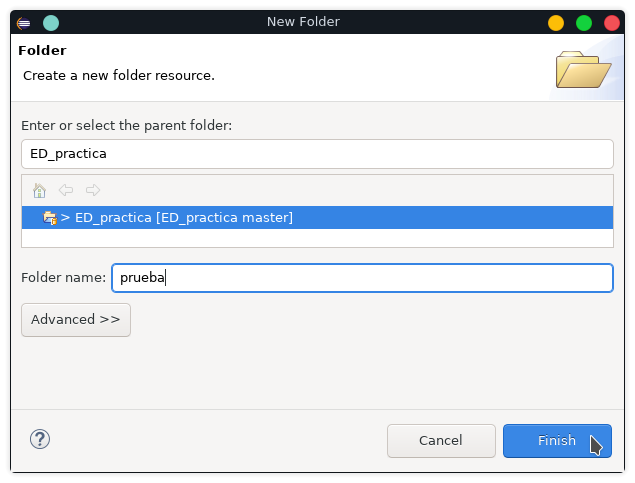
\includegraphics[scale=0.75]{./Pictures/023_prueba_dir.png}
\end{figure}

En esta parte es importante desactivar la opción \textbf{Use default location}
y colocar la ruta donde se encuentra el proyecto y la carpeta específica donde
vas a guardar el proyecto. Para esto en el paso anterior creamos una carpeta
llamada prueba.\\

\begin{figure}[h!]
  \centering
  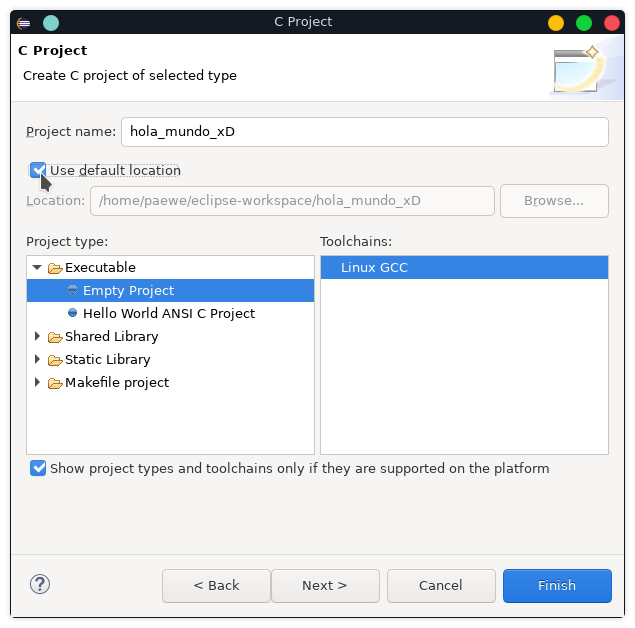
\includegraphics[scale=0.75]{./Pictures/022_desmarcar.png}
\end{figure}

\newpage

Por esto mi ruta quedaría: \textbf{route-to/ED\_practica/prueba}. Aquí
\textbf{route-to} es la ruta hasta donde se encuentra el directorio del proyecto
clonado que en este caso particular se llama \textbf{ED\_prueba} y nuestro
proyecto anidado se guardará en el directorio \textbf{prueba}.\\

También hay que diferenciar que el nombre del proyecto, que para este caso
particular es \textbf{hola\_mundo\_xD} está guardándose en el directorio
\textbf{prueba}. Un poco confuso lo sé, pero si no entienden muy bien esto me
preguntan con toda confianza.

\begin{figure}[h!]
  \centering
  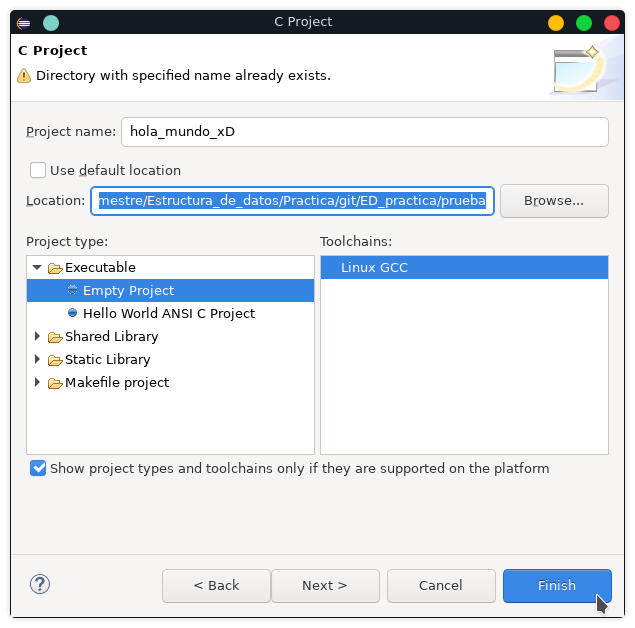
\includegraphics[scale=0.75]{./Pictures/023_new_project.png}
\end{figure}

Ahora en el proyecto \textbf{hola\_mundo\_xD} vamos a crear un directorio
\textbf{src} (en la práctica se estará creando un directorio \textbf{src}
dentro de \textbf{prueba}).

\begin{figure}[h!]
  \centering
  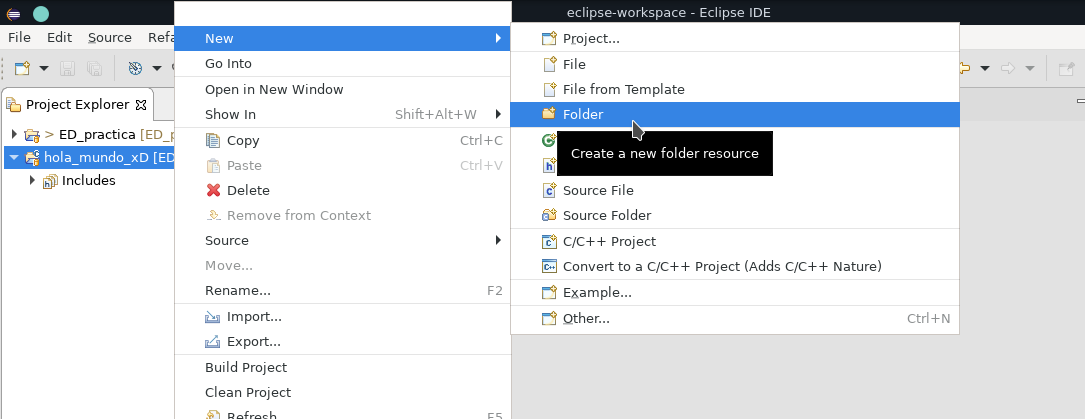
\includegraphics[scale=0.65]{./Pictures/024_hola_mundo_xD_dir.png}
\end{figure}

\newpage

\begin{figure}[h!]
  \centering
  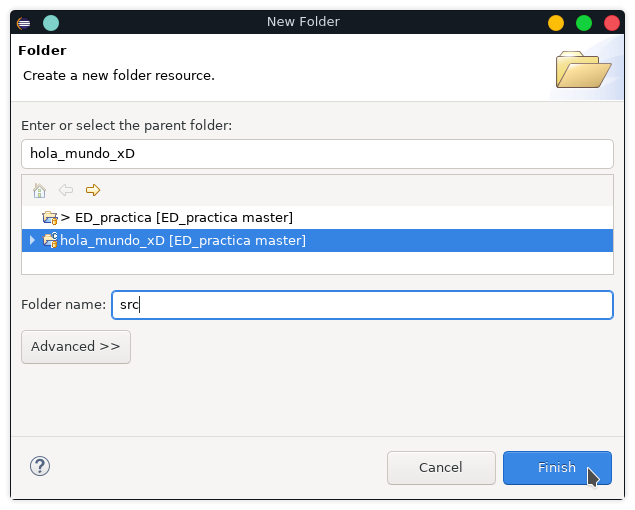
\includegraphics[scale=0.75]{./Pictures/025_src.png}
\end{figure}

En \textbf{src} vamos a crear un nuevo fichero de tipo C para realizar
finalmente el programa.

\begin{figure}[h!]
  \centering
  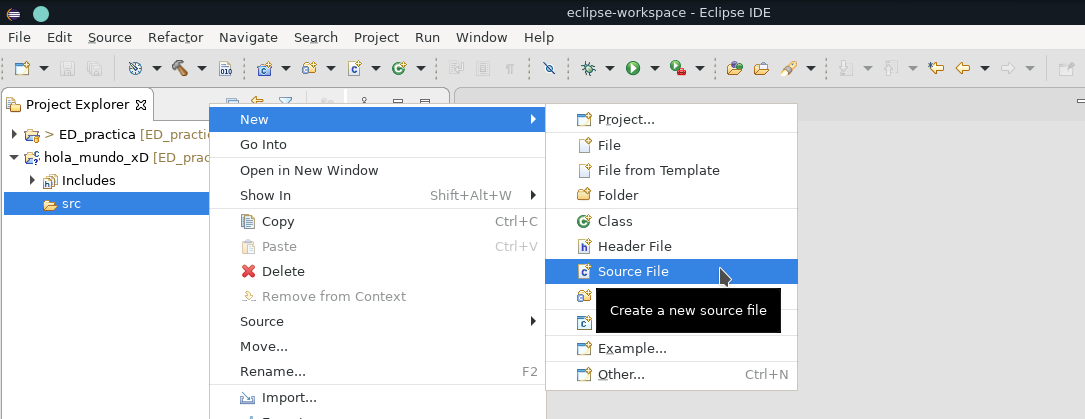
\includegraphics[scale=0.65]{./Pictures/026_new_c_file.png}
\end{figure}

\begin{figure}[h!]
  \centering
  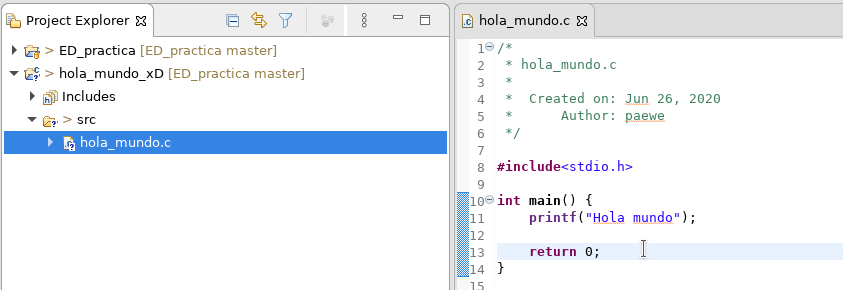
\includegraphics[scale=0.75]{./Pictures/027_hola_mundo.png}
\end{figure}

\newpage

Para correr el programa se puede usar la opción \textbf{Build Project} o como
se muestra en la captura.

\begin{figure}[h!]
  \centering
  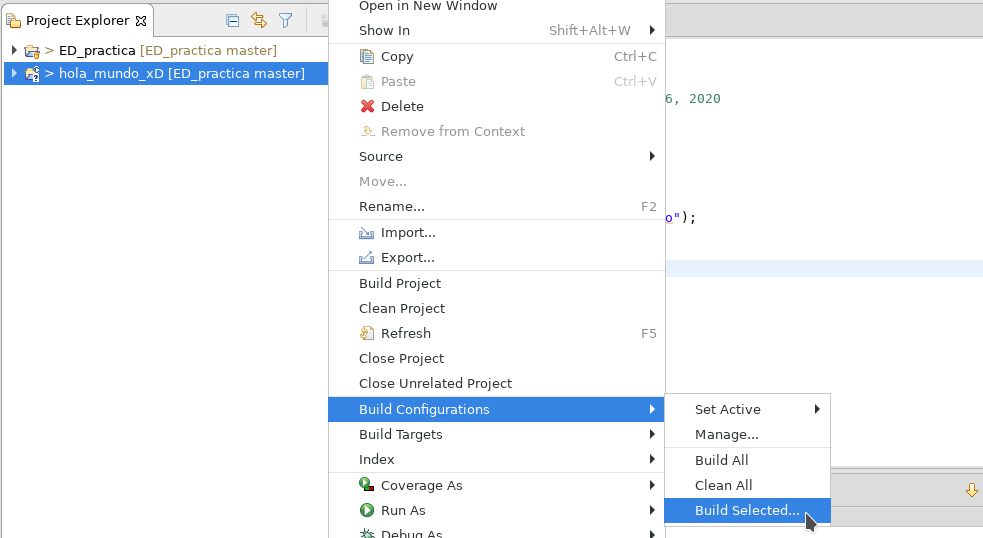
\includegraphics[scale=0.65]{./Pictures/028_build_selected.png}
\end{figure}

\begin{figure}[h!]
  \centering
  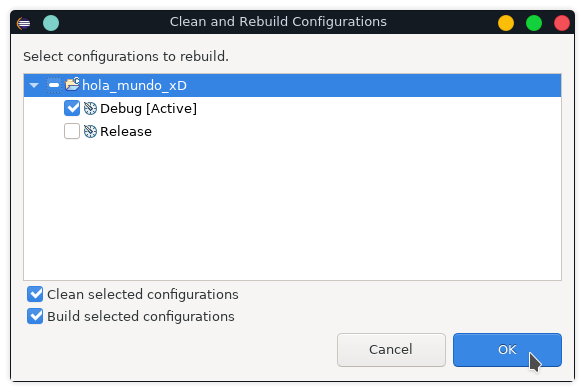
\includegraphics[scale=0.75]{./Pictures/029_clean_rebuild.png}
\end{figure}

Esto va a crear una carpeta llamada \textbf{Debug} donde estará el binario
compilado. Ahora ya se puede ejecutar el programa. Ahi dejo dos formas.

\begin{figure}[h!]
  \centering
  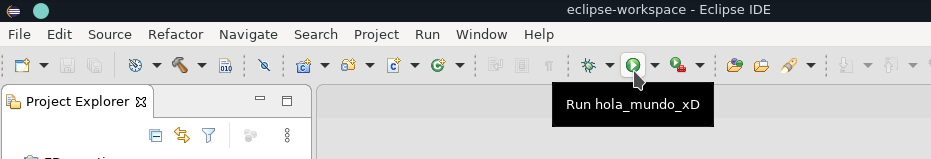
\includegraphics[scale=0.75]{./Pictures/029_run_bitch.png}
\end{figure}

\newpage

\begin{figure}[h!]
  \centering
  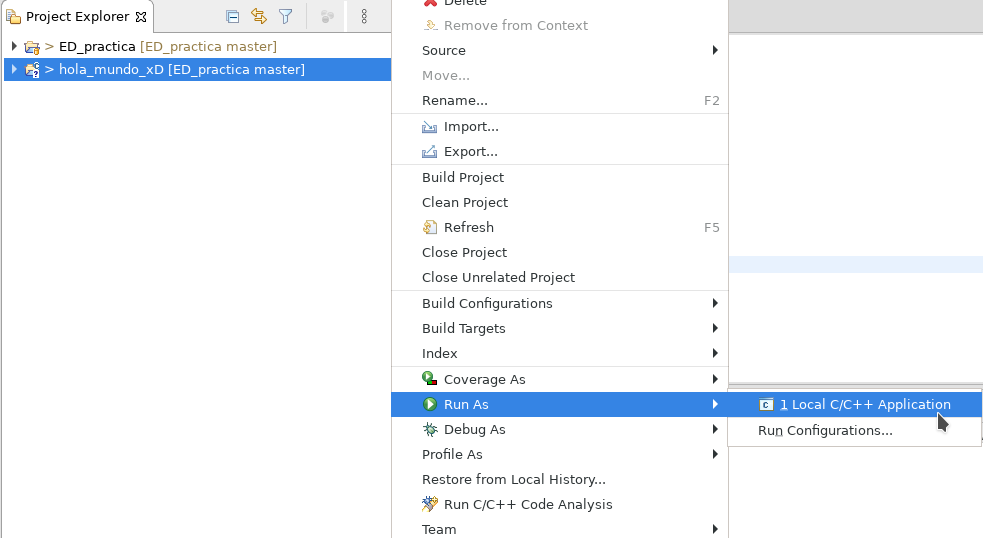
\includegraphics[scale=0.65]{./Pictures/029_hola_mundo_ejecutado.png}
\end{figure}

\begin{figure}[h!]
  \centering
  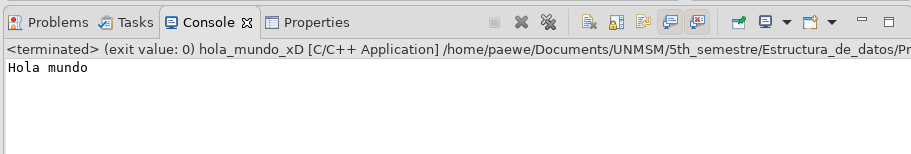
\includegraphics[scale=0.75]{./Pictures/030_ejecutado.png}
\end{figure}


\newpage

\subsection*{Subiendo cambios del repositorio local al remoto con Eclipse}%
Por último en esta parte les quiero mostrar cómo subir los cambios al
repositorio del que o tienes que ser dueño o colaborador. En mi caso, el
repositorio lo cree así que soy dueño.\\

Algunos podrán pensar que hacer esto gráficamente no tiene tanto gusto como
cuando lo realizas por terminal (yo prefiero la terminal), pero a veces es
bastante útil la agilidad que te brinda Eclipse cuando se trata de hacer
commits en un repositorio local y luego mandarlo al remoto.\\

Por ejemplo aquí hice captura de cuando envié la tarea xd:\\

Primero mostramos el panel \textbf{Git Staging}.
\begin{figure}[h!]
  \centering
  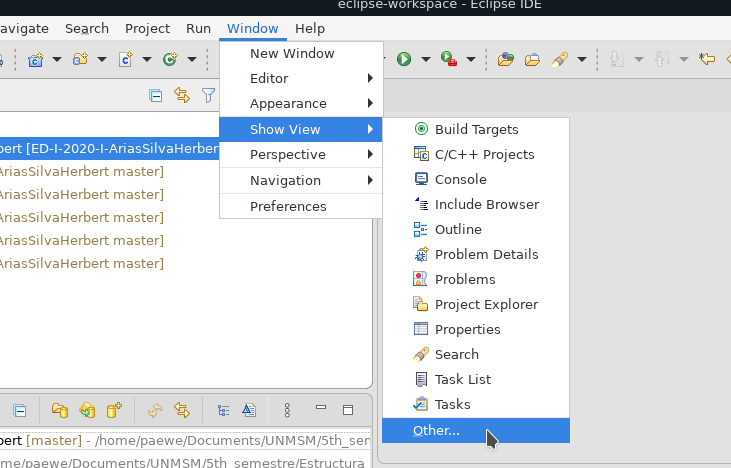
\includegraphics[scale=0.75]{./Pictures/031_show_view_git_stash.png}
\end{figure}

\begin{figure}[h!]
  \centering
  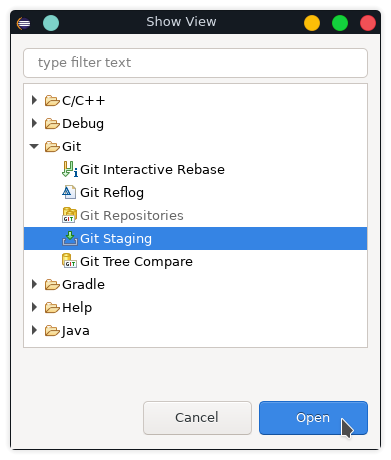
\includegraphics[scale=0.75]{./Pictures/032_git_staging.png}
\end{figure}

\newpage

Esto es como hacer: \textbf{git add -A}

\begin{figure}[h!]
  \centering
  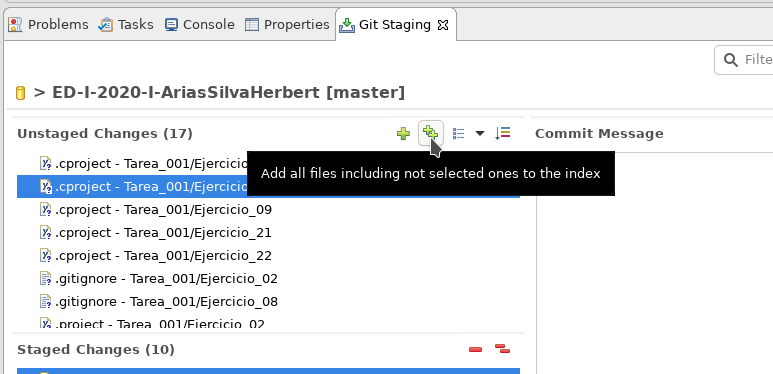
\includegraphics[scale=0.75]{./Pictures/033_git_add_all.png}
\end{figure}

Y esto como hacer: \textbf{git commit} y todo el mensaje. Además de \textbf{git
push origin master}

\begin{figure}[h!]
  \centering
  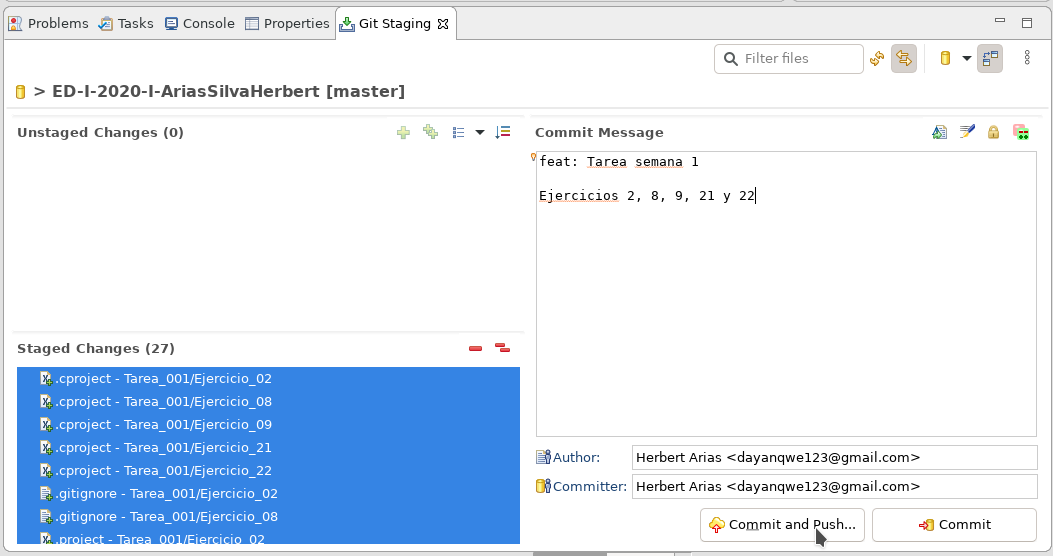
\includegraphics[scale=0.65]{./Pictures/034_git_commit_and_push.png}
\end{figure}

\begin{figure}[h!]
  \centering
  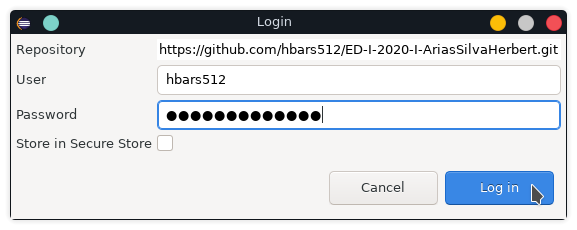
\includegraphics[scale=0.75]{./Pictures/035_login_sent.png}
\end{figure}

\newpage

\begin{figure}[h!]
  \centering
  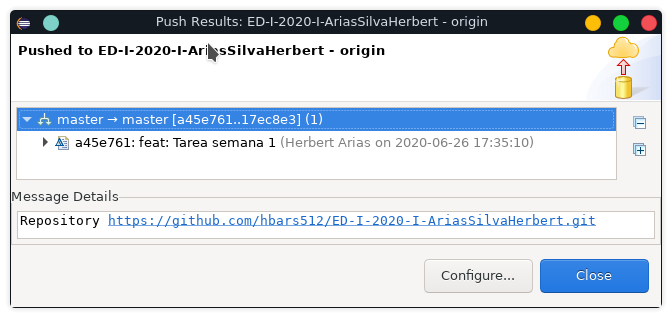
\includegraphics[scale=0.75]{./Pictures/036_push_results.png}
\end{figure}

\end{document}

